
\section{Les règles}
\lettrine{L}{es} règles de \swfe sont particulièrement simples et suivent un modèle commun. Rentrons dans le vif du sujet et voyons comment ça fonctionne.

\subsection{Les Traits}
Chaque personnage ou créature a deux types de Traits, les Attributs et les Compétences. Chaque Trait a un score allant de d4 à d12, d6 étant la moyenne.

\subsubsection{Tests}
Quand vous voulez faire quelque chose, le MJ vous dit quel Trait vous devez utiliser, et vous lancez le dé correspondant. Si le résultat est de 4 ou mieux, une fois les modificateurs appliqués, alors l’action est réussie. Certains personnages ou créatures ont des Traits supé- rieurs à d12, comme d12+3. Cela signifie qu’il faut lancer un d12, puis ajouter 3.

\begin{description}
\item[Difficulté :] La Difficulté pour la plupart des actions est 4, plus ou moins les modificateurs. La Parade et la Résistance constituent des Difficulté spéciales qui seront expliquées plus tard.

\item[Compétence par défaut :] Si un personnage ne dispose pas de la compétence nécessaire à une action, il tire 1d4 et enlève 2 au total. Certaines compétences ne peuvent pas être utilisées par défaut, comme lancer un sort ou procéder à une intervention chirurgicale à cerveau ouvert.
\end{description}

\subsubsection{As}
Les jets de Traits et de dégâts dans \swfe sont dits “ouverts”. Cela signifie que lorsque vous tirez le maximum du dé (un 6 sur un d6, un 8 sur un d8, etc.), vous relancez le dé et l’ajoutez au total. C’est ce qu’on appelle un “As“, et vous continuez à additionner les résultats tant que vous obtenez des As !

\subsubsection{Relances}
Parfois, il est important de savoir à quel point une action est réussie. Pour chaque tranche de 4 points au-dessus de la Difficulté, on obtient une Relance. Si votre héros a besoin d’un 4 pour toucher un adversaire et qu’il obtient un 8, il touche avec une Relance.

\begin{commentbox}{Exemple}
Une chasseuse de prime a une Difficulté de 4 pour toucher le Tusken à portée courte avec son Pistolet blaster. Elle a d8 en Tir, tire donc un dé à 8 faces, et obtient un 8. C’est un As, aussi tire-telle le dé à nouveau pour obtenir un 4, pour un total de 12. Elle obtient donc deux Relances.
\end{commentbox}

\subsubsection{Jets opposés}
Parfois, les jets se font “en opposition“ contre un adversaire. Par exemple, si deux personnages luttent à mains nues pour s’emparer d’un artefact ancien, ils font chacun un jet de Force. Quand ce genre de cas se présente, le personnage actif fait son jet en premier, suivi par l’adversaire qui lui résiste. Le plus haut résultat l’emporte.

\begin{commentbox}{Exemple}
Ubbal Zherooh, un marchand, tente une négociation sur un Jawa. Ubbal obtient un 7 sur son jet de Persuasion. Le Jawa réfléchit et obtient un 3 sur son jet de Persuasion. Ubbal remporte le deal avec une Relance !
\end{commentbox}


\subsection{Jokers \& extras}
Votre héros (un personnage joueur) et certains grands méchants et monstres sont dénommés « Jokers ». Ces personnages ont de meilleures chances que les autres de réussir ce qu’ils entreprennent, sont un peu plus résistants et généralement plus détaillés que ne le sont de simples gardes, sbires ou laquais (les « Extras »).

\subsubsection{Le Dé Joker}
Lors d’un jet de Trait, quel qu’il soit, les Jokers lancent un d6 supplémentaire et prennent le meilleur des deux jets entre le jet de Trait et de le Dé Joker. Les As et tout modificateur s’appliquent aussi au Dé Joker.

\begin{description}
\item[Un dé joker par action :] quand un Joker tire plusieurs dés au cours d’une même action, comme lors d’un tir automatique, il ne tire qu’un seul Dé Joker. Un tireur qui tire 3 balles par exemple, lance 3 fois son dé de Tir, et une seule fois son Dé Joker, qui peut alors se substituer à l’un des jet de tir, s’il est supérieur.
\end{description}

\begin{commentbox}{Exemple}
Un héros avec d8 en Force fait un jet. Il lance donc un d8 et son Dé Joker, un d6, et obtient respectivement 8 et 6 — c’est un As sur chacun des dés ! Il lance à nouveau les deux dés, et obtient 4 et 3. Le d8 totalise donc 8+4=12, alors que le Dé Joker totalise 6+3=9. Le d8 a obtenu le meilleur score final, dans ce cas, le total est 12.
\end{commentbox}

\subsubsection{Jetons}
\swfe offre aux joueurs et MJs un peu de contrôle sur les caprices du destin. Chaque joueur commence ainsi une session de jeu avec trois Jetons, matérialisés par des jetons ou des pions quelconques, qui représentent un peu de la chance des héros ou le destin. Vous pouvez utiliser ces Jetons pour retirer tout jet de Trait. Vous pouvez même le faire plusieurs fois si ça vous chante, jusqu’à obtenir le résultat souhaité tant qu’il vous reste des Jetons. Vous gardez toujours le meilleur des jets – utiliser un Jeton ne devrait jamais faire tourner une action en désastre. Si votre premier jet était un 5, et que le Jeton vous donne un 4, vous conservez le 5.

Les Jetons ne peuvent pas être utilisés pour les jets de dégâts, les jets sur des tables et tout jet autre qu’un jet de Trait (les Jet d’encaissement et certains Atouts permettent d’utiliser des Jetons pour autre chose que des jets de Trait, mais il s’agit d’exceptions). Les Jetons ne sont pas conservés d’une session sur l’autre, utilisez-les ou dites-leur au revoir.

\subsubsection{Jetons du MJ}
Les MJ ont aussi des Jetons pour leurs méchants. Au début de chaque session de jeu, il en récupère un pour chaque joueur qui compose le groupe, et deux de plus par Joker qu’il contrôle. Ces derniers peuvent s’en servir pour sauver leurs sales peaux plutôt que de puiser dans les Jetons du MJ. Et non, ils ne peuvent pas les prêter à leurs sbires. Comme pour les héros, ces Jetons ne sont pas conservés d’une session sur l’autre.

\begin{tikzpicture}[overlay, remember picture]
\node[anchor=south, %anchor is upper left corner of the graphic
      xshift=0, %shifting around
      yshift=3cm] 
     at (current page.south) %left upper corner of the page
     {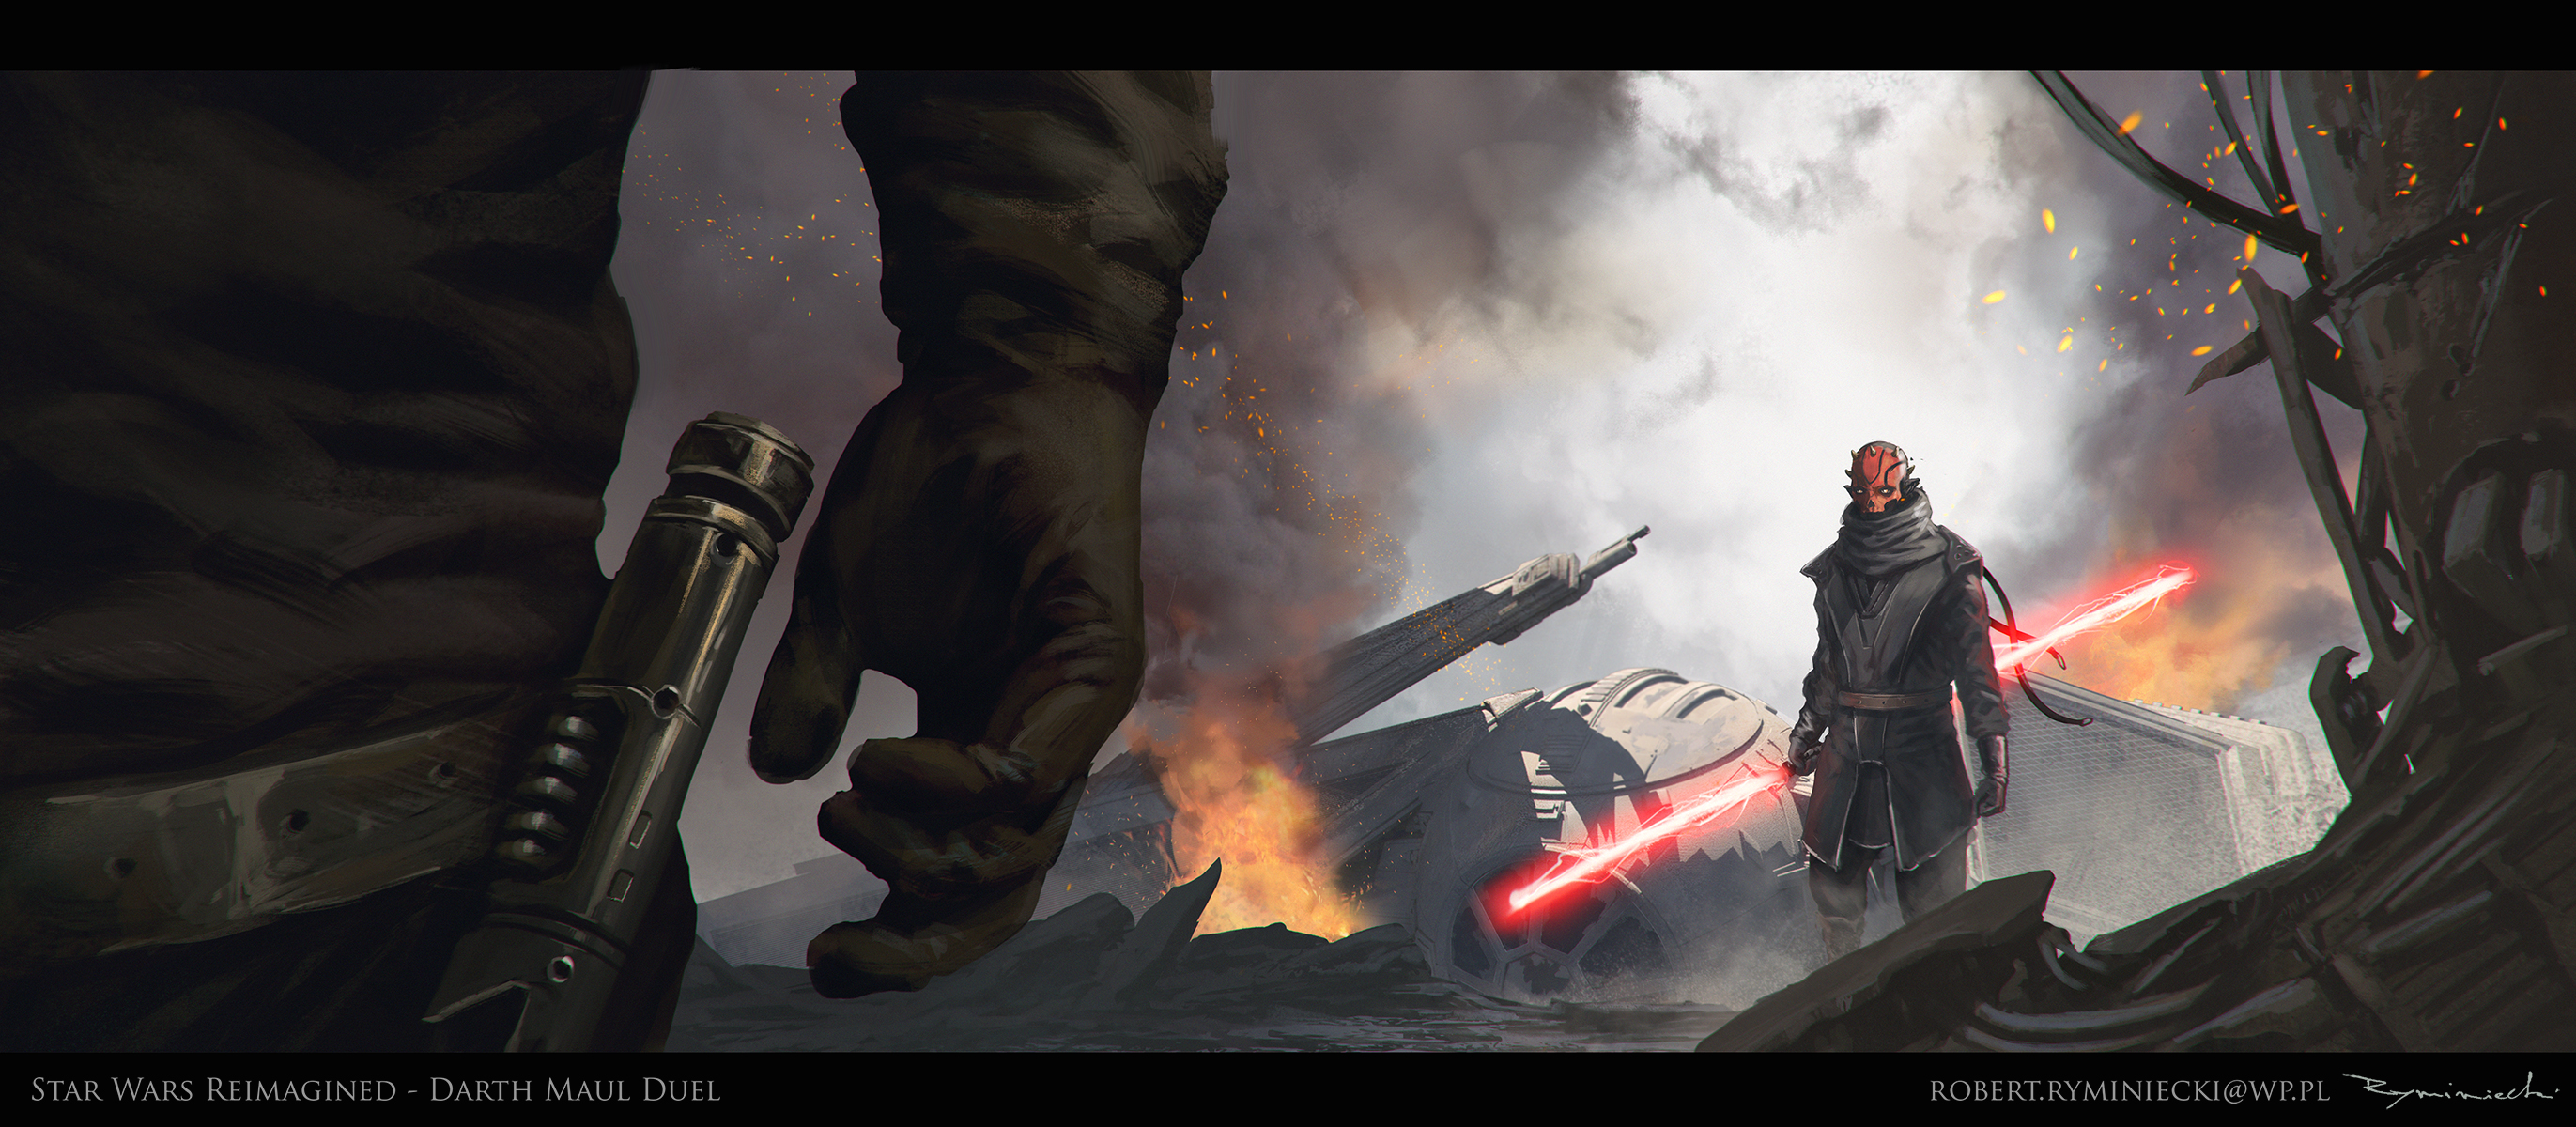
\includegraphics[width=\textwidth]{img/starwars_redesign_final_by_rymin07-d9pqtj6.jpg}}; 
\end{tikzpicture}